% !TEX root = ./document.tex

\documentclass[a4paper, spanish]{article}

\usepackage{mystyle}
\usepackage{myvars}
\usepackage{mylinearprogramming}
%-----------------------------


\begin{document}

  \maketitle

  \abstract \noindent Los problemas de abastecimiento de producto son un problema constante para nuestra sociedad. Es por ello que la modelización adecuada de los mismos para su estudio y resolución de manera eficiente debe ser estudiada en detalle. Por tanto, en este trabajo se analiza la modelización del problema multiproducto de suministrar existencias a destinos con determinadas necesidades a partir de orígenes con determinadas demandas pasando por puntos intermedios con restricciones de capacidad también determinadas. Dicha problemática se estudia a mediante la modelización de \emph{Programación Lineal}, \emph{Transporte en 2 Etapas} y \emph{Flujo de Redes}.

  %-----------------------------
  %  TEXT
  %-----------------------------

  \section{Introducción}

    \paragraph{}
    En este documento se va a estudiar el planteamiento del problema del transporte de mercancías desde un conjunto de orígenes hacia un conjunto de destinos, los cuales deben visitar un almacen intermedio. En este caso, el contexto del problema es el siguiente: \emph{La empresa transeuro quiere encontrar la solución óptima para transportar sus mercancías de dos tipos $\{p_1, p_2\}$ desde los puntos de origen $I = \{i_1, i_2\}$ hacia los puntos de destino $J = \{j_1, j_2, j_3\}$ teniendo que atravesar obligatoriamente uno de los puntos intemedio $W =\{w_1, w_2\}$. En el problema, el conjunto $I$ se refiere a puertos de origen,el conjunto $W$ a almacenes intermedio y el conjunto $J$ a ciudades de destino. Cada puerto de origen tiene una determinada cota de producción por producto (que denotaremos por $s_{ik}$), y cada destino una determinada demanda por producto (que denotaremos por $d_{jk}$). Además, cada almacen impone una restricción de espacio total (que denotamos por $u_{w}$). En cuanto a los costes de transporte, este tan solo depende de la ruta y se mantiene constante para el producto, por lo que lo denotaremos por $c_{ij}$}. (Los valores concretos utilizados pueden ser consultados en el Apéndice \ref{appendix:data}).

    \paragraph{}
    Puesto que el objetivo de este trabajo reside en la comparación de las distintas modelizaciones posibles para resolver el problema, esta notación variará en ciertas ocasiones para adaptarse a las restricciones específicas de cada problema. Para tratar de facilitar al máximo la comparación entre modelos por parte del usuario, se ha decidido utilizar tan solo una representación en el conjunto de datos (sin que este tenga que tener en cuenta el balanceo del problema cuando el modelo lo requiere). A costa de esto, se ha añadido cierta complejidad en la lectura de datos, que requiere de la adaptación concreta hacia la entrada necesaria para cada modelo.

    \paragraph{}
    El conjunto de datos puede visualizarse mediante su representación en forma de grafo en la figura \ref{img:graph-network}, en la cual se incluyen los vértices o puntos que representan, orígenes, almacenes y destinos, así como la oferta y demanda de cada uno de ellos, junto con las restricciones de capacidad y los costes de cada arista.

    \begin{figure}[!hp]
      \centering
      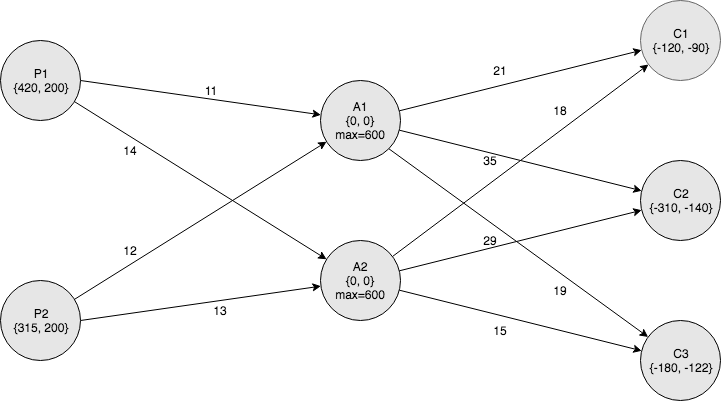
\includegraphics[width=0.7\textwidth]{cost-demand-capacity}
      \caption{Representación gráfica del Conjunto de Datos}
      \label{img:graph-network}
    \end{figure}

    \paragraph{}
    El resto del documento se organiza de la siguiente manera: se describen los tres modelos estudiados (\emph{Programación Lineal} en la sección \ref{section:linear-programming}, \emph{Transporte en 2 Etapas} en la sección \ref{section:transportation} y \emph{Flujo de Redes} en la sección \ref{section:network-flow}) en las cuales se hace especial incapié en las dificultades de implementación así como el coste computacional y las restricciones propias del modelo en caso de ser necesarias. Para finalizar, en la sección \ref{section:conclusions} se concluye el trabajo con una comparación global entre las tres estrategias de modelización.

  \section{Planteamiento: Programación Lineal}
  \label{section:linear-programming}

    \paragraph{}
    El modelo de programación lineal es el más sencillo de entender a nivel conceptual de entre los que se estudian en este trabajo. Este modelo se muestra en la ecuación \eqref{eq:linear-programming-model}. Se basa en un conjunto de variables indexadas en 4 índices (referidos a origen, destino, almacén y producto), indicando cada variable la cantidad de producto que se envía por cada camino posible. Para ello, tan solo es necesario la cantidad máxima de producto en el origen (mediante la primera restricción), el cubrimiento de unidades de producto en los destinos (mediante la segunda restricción) y las limitaciones de producto total por almacén (mediante la tercera restricción). Es trivial entender la última restricción de no negatividad.

    \begin{eqfloat}
      \begin{equation}
        \begin{array}{ll@{}ll}
          \text{Minimizar}	& \displaystyle \sum\limits_{i=1}^{n}\sum\limits_{j=1}^{m}\sum\limits_{w=1}^{l}\sum\limits_{k=1}^{p} x_{ijwk} \cdot c_{ijw} \\
          \text{sujeto a}		& \sum\limits_{j=1}^{m}\sum\limits_{w=1}^{l} x_{ijwk}	\leq s_{ik}, 		& \forall i \in \{1,...,n\}, \forall k \in \{1,...,p\}\\
                            &	\sum\limits_{i=1}^{n}\sum\limits_{w=1}^{l} x_{ijwk}	\geq d_{jk}, 		& \forall j \in \{1,...,m\}, \forall k \in \{1,...,p\}\\
                            &	\sum\limits_{i=1}^{n}\sum\limits_{j=1}^{m}\sum\limits_{k=1}^{p} x_{ijwk}	\leq u_{w}, 		& \forall w \in \{1,...,l\}  \cap u_{w} > 0 \\
                            & x_{ijwk}	\geq 0, 	& \forall i \in \{1,...,n\}, \forall j \in \{1,...,m\}, \forall w \in \{1,...,l\}, \forall k \in \{1,...,p\}
        \end{array}
      \end{equation}
      \caption{Formulación como \emph{Problema de Programación Lineal}.}
      \label{eq:linear-programming-model}
    \end{eqfloat}

    \paragraph{}
    Nótese que en este caso no es necesario balancear el problema, puesto que no estamos imponiendo ninguna restricción de igualdad que \say{obligue} a transportar todo el producto. Nos podemos permitir dicha ventaja porque en este modelo no existe la posibilidad de que quede mercancia por los puntos intermedios del camino (algo que no siempre sucederá como veremos en el modelo de \emph{Flujo de Redes} de la sección \ref{section:network-flow}).

    \paragraph{}
    En cuanto al número de variables de decisión necesarias para resolver el problema, en este caso necesitamos $n(I) \cdot n(J) \cdot n(W) \cdot n(P) = 2 \cdot 3 \cdot 2 \cdot 2 = 24$. A nivel de restricciones, tenemos $n(I) \cdot n(P) + n(W) \cdot n(P) + n(J) \cdot n(P) + \cdot n(W) + n(I) \cdot n(J) \cdot n(W) \cdot n(P) = 2 \cdot 2 + 2 \cdot 2 + 3 \cdot 2 + 2 \cdot 3 \cdot 2 \cdot 2 = 38$. En la implementación realizada cuyo código fuente puede ser consultado en el Apéndice \ref{appendix:source-code-linear-programmming} se ha encontrado la solución óptima en 11 iteracciónes.

    \begin{figure}[!hp]
      \centering
      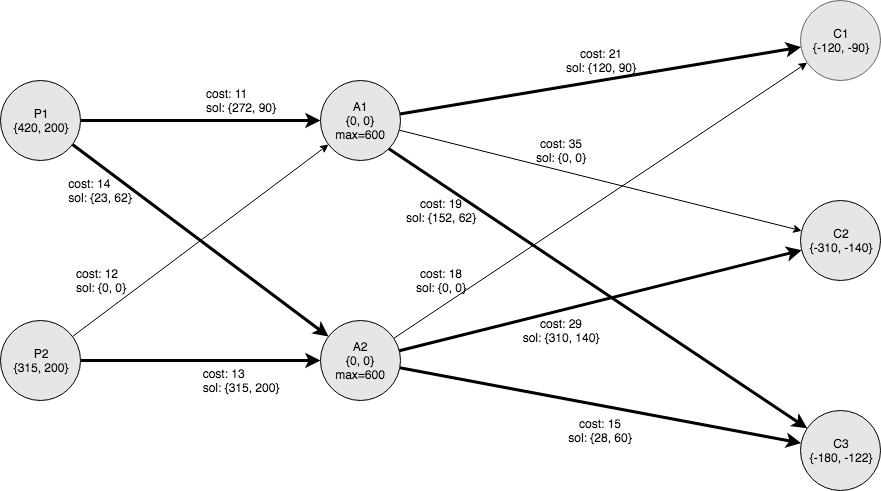
\includegraphics[width=0.8\textwidth]{linear-programming}
      \caption{Representación gráfica de la solución obtenida mediante la modelización como problema de \emph{Programación Lineal}}
      \label{img:graph-linear-programming}
    \end{figure}

    \paragraph{}
    La solución obtenida mediante la modelización como un problema de programación lineal se muestra en la figura \ref{img:graph-linear-programming}.


  \section{Planteamiento: Transporte en 2 Etapas}
  \label{section:transportation}

    \paragraph{}
    Con el modelo de transporte se posee la ventaja de conocer algoritmos muy eficientes para su resolución. Sin embargo, estos están planteados para problemas \say{directos}, es decir, aquellos en los cuales tan solo se tiene orígenes, destinos y un único producto. Por lo tanto, para modelizar nuestro problema de esta manera debemos realizr una serie de modificaciones. Este modelo se muestra en la ecuación \eqref{eq:transportation-model}.

    \paragraph{}
    La primera de ellas se basa en el desdoble del problema en dos etapas, para así obtener dos problemas que cumplirían las especificaciones del modelo de transporte si se desdoblan por productos. Por tanto, utilizaremos dos conjuntos de variables indexadas en tres índices y denotadas como $x^{1}_{iwk}$ para representar la cantidad de producto $k$ del origen $i$ al almacén $w$ y $x^{2}_{wjk}$ para representar la cantidad de producto $k$ del almacén $w$ al destino $j$.

    \paragraph{}
    Al igual que en el caso anterior, es necesario imponer la restricción máxima de producción sobre los orígenes (mediante la primera restricción), así como la \say{conexión} de los dos conjuntos de variables en los almacenes (mediante la segunda restricción). Lo siguiente es imponer las restricciones de demanda sobre los origines (tal y como se puede ver en la tercera restricción). Por último, es necesario añadir la restricción de capacidad, que en este caso se podría realizar sobre cualquiera de los dos conjuntos de variables (por estar en los almacenes), pero parece más razonable incluirla sobre el primer conjunto (tal y como se ha hecho en la cuarta restricción). Es trivial entender las dos últimas restricciones de no negatividad.

    \paragraph{}
    En este caso tampoco es necesario balancear el problema siguiendo el mismo planteamiento que en el caso anterior, ya que por la relación de transitividad entre las dos etapas del problema de transporte, este hará los excedentes de producto queden en el origen.

    \begin{eqfloat}
      \begin{equation}
        \begin{array}{ll@{}ll}
          \text{Minimizar}	& \displaystyle \sum\limits_{i=1}^{n}\sum\limits_{w=1}^{l}\sum\limits_{k=1}^{p} x^{1}_{iwk} \cdot c^{1}_{iw} +
              \sum\limits_{w=1}^{l}\sum\limits_{j=1}^{m}\sum\limits_{k=1}^{p} x^{2}_{wjk} \cdot c^{2}_{wj} \\
          \text{sujeto a}		& \sum\limits_{w=1}^{l} x^{1}_{iwk}	\leq s_{ik}, 		                        & \forall i \in \{1,...,n\}, \forall k \in \{1,...,p\}\\
                            &	\sum\limits_{i=1}^{n} x^{1}_{iwk}	= \sum\limits_{j=1}^{m} x^{2}_{wjk}, 		& \forall w \in \{1,...,l\}, \forall k \in \{1,...,p\}\\
                            &	\sum\limits_{w=1}^{l} x^{2}_{wjk}	\geq d_{jw}, 		                        & \forall j \in \{1,...,m\}, \forall k \in \{1,...,p\}\\
                            &	\sum\limits_{i=1}^{n}\sum\limits_{k=1}^{p}  x^{1}_{iwk}	\leq u_{w}, 		  & \forall w \in \{1,...,l\} \cap u_{w} > 0\\
                            & x^{1}_{iwk}	\geq 0, 	& \forall i \in \{1,...,n\}, \forall w \in \{1,...,l\}, \forall k \in \{1,...,p\} \\
                            & x^{2}_{wjk}	\geq 0, 	& \forall w \in \{1,...,l\}, \forall j \in \{1,...,m\}, \forall k \in \{1,...,p\}
        \end{array}
      \end{equation}
      \caption{Formulación como \emph{Problema de Transporte en 2 Etapas}.}
      \label{eq:transportation-model}
    \end{eqfloat}

    \paragraph{}
    En cuanto al número de variables de decisión necesarias para el planteaminento del modelo, en este caso han utilizado $n(I) \cdot n(W) \cdot n(P) + n(W) \cdot n(J) \cdot n(P) = 2 \cdot 2 \cdot 2 + 2\cdot 3\cdot 2 = 8 + 12 = 20$ junto con $n(I) \cdot n(P) + n(W) \cdot n(P) + n(J) \cdot n(P) + n(W) + n(I) \cdot n(W) \cdot n(P) + n(W) \cdot n(J) \cdot n(P) = 2 \cdot 2 + 2 \cdot 2 + 3 \cdot 2 + 2 + 2 \cdot 2 \cdot 2 +  2 \cdot 3 \cdot 2 = 36$. En la implementación cuyo código fuente puede ser consultado en el Apéndice \ref{appendix:source-code-transportation} realizada se ha encontrado la solución óptima en 14 iteracciónes.

    \begin{figure}[!hp]
      \centering
      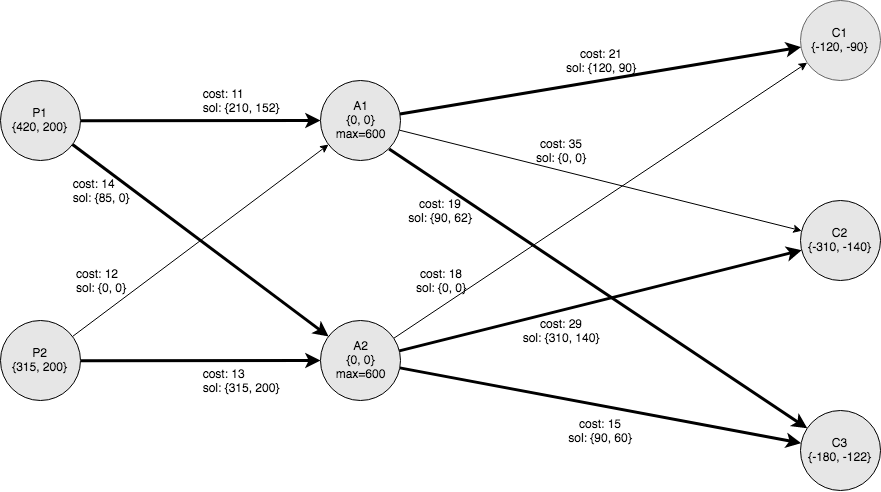
\includegraphics[width=0.8\textwidth]{transportation}
      \caption{Representación gráfica de la solución obtenida mediante la modelización como problema de \emph{Transporte en 2 Etapas}}
      \label{img:graph-transportation}
    \end{figure}

    \paragraph{}
    La solución obtenida mediante la modelización como un problema de transporte se muestra en la figura \ref{img:graph-transportation}.


  \section{Planteamiento: Flujo de Redes}
  \label{section:network-flow}

    \paragraph{}
    El último modelo que se analizará en este trabajo es el basado en  flujo de redes. Este se diferencia de los anteriores porque no impone ninguna restricción con respecto a orígenes, destinos o puntos intermedios, sino que todos son equivalentes. Sin embargo, para que esta modelización sea apropiada el problema debe ser balanceado, ya que lo que se busca es el punto de equilibrio entre las necesidades de todos los vértices.  Este modelo se muestra en la ecuación \eqref{eq:network-flow-model}.

    \paragraph{}
    Por tanto, en este caso es necesario balancear el problema (que en el caso de la implementación actual se hace automáticamente). Sin embargo, lo haríamos de manera manual sería incluir un nuevo conjunto de aristas de coste cero conectadas a los vértices productores con demanda equivalente al opuesto del excedente. Es decir, $d_{81} = -125, d_{82} = -48$.

    \paragraph{}
    En cuanto a las restricciones necesarias para el modelo, puesto que lo que se busca es la estabilidad es necesario codificar la capacidad y demanda en un único vector al que denominaremos $d$ siendo $d_{i}$ la demanda (con signo negativo para los vértices consumidores), la oferta (con signo positivo para los vértices productores) y 0 en caso de que sean vértices de \say{paso}. Lo siguiente es igualar la entrada menos la salida a este valor (tal y como se hace en la primera restricción). En cuanto a las capacidades, basta con restringir el valor de entrada (o salida) a la capacidad del máxima del vértice (como se indica en la segunda restricción). La última restricción de positividad es trivial.

    \begin{eqfloat}
      \begin{equation}
        \begin{array}{ll@{}ll}
          \text{Minimizar}	& \displaystyle \sum\limits_{i=1}^{n}\sum\limits_{j=1}^{n}\sum\limits_{k=1}^{p} x^{1}_{ijk} \cdot c_{ij} \\
          \text{sujeto a}		& \sum\limits_{j=1}^{n} x^{1}_{ijk} - \sum\limits_{j=1}^{n} x^{1}_{jik} = d_{ik}, & \forall i \in \{1,...,n\}, \forall k \in \{1,...,p\}\\
                            &	\sum\limits_{j=1}^{n}\sum\limits_{k=1}^{p}  x_{ijk}	\leq u_{i}, 		  & \forall i \in \{1,...,l\} \cap u_{i} > 0\\
                            & x_{ijk}	\geq 0, 	& \forall i \in \{1,...,n\}, \forall j \in \{1,...,n\}, \forall k \in \{1,...,p\}
        \end{array}
      \end{equation}
      \caption{Formulación como \emph{Problema Flujo de Redes}.}
      \label{eq:network-flow-model}
    \end{eqfloat}

    \paragraph{}
    En cuanto al número de variables de decisión necesarias para el planteaminento del modelo, en este caso han utilizado $ (n(I) + n(I) + n(W) + 1) \cdot n(P) = 8 \cdot 2 = 16$ junto con $(n(I) + n(I) + n(W) + 1) \cdot n(P) + (n(I) + n(I) + n(W) + 1) + (n(I) + n(I) + n(W) + 1) \cdot n(P) = 16 + 8 + 16 = 40$. En la implementación cuyo código fuente puede ser consultado en el Apéndice \ref{appendix:source-code-network-flow} realizada se ha encontrado la solución óptima en 10 iteracciónes.


    \begin{figure}[!hp]
      \centering
      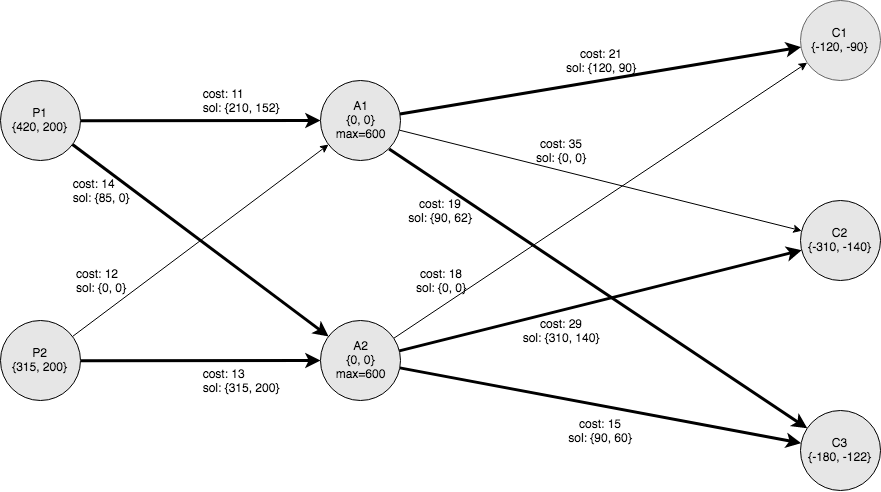
\includegraphics[width=0.8\textwidth]{network-flow}
      \caption{Representación gráfica de la solución obtenida mediante la modelización como problema de \emph{Flujo de Redes}}
      \label{img:graph-network-flow}
    \end{figure}

    \paragraph{}
    La solución obtenida mediante la modelización como un problema de flujo de redes se muestra en la figura \ref{img:graph-network-flow}.

  \section{Conclusiones}
  \label{section:conclusions}

    \paragraph{}
    A partir de las tres modelizaciones se obtiene el resultado óptimo para la planificación del problema (coste de \textbf{$34465$}). Sin embargo, esta solución no es única, ya tal y como se ha visto en los resultados, a pesar de que estos no son iguales para los tres modelos, el valor óptimo si que lo es. A nivel de complejidad computacional, el la modelización de flujos de redes parece el más eficiente de los tres pagando el precio de la necesidad de balanceo previo.

    \paragraph{}
    Sería interesante comparar dichas soluciones sobre un conjunto de datos de tamaño mayor para comprobar la eficiencia de cada modelización, así como su comparación con soluciones basadas en heurísticas.

  \begin{appendices}

    \section{Código Fuente}

      \subsection{Programación Lineal}
      \label{appendix:source-code-linear-programmming}

        \inputminted{text}{./../mosel/linear-programming-model.mos}

      \subsection{Transporte en 2 Etapas}
      \label{appendix:source-code-transportation}

        \inputminted{text}{./../mosel/two-steps-transportation-model.mos}

      \subsection{Flujo de Redes}
      \label{appendix:source-code-network-flow}

        \inputminted{text}{./../mosel/network-flow-model.mos}

    \section{Datos}
    \label{appendix:data}

      \inputminted{text}{./../mosel/data.dat}

  \end{appendices}





  %-----------------------------
  %  Bibliographic references
  %-----------------------------

  \nocite{subject:pent2017}
  \nocite{tool:xpress-mosel}
  \nocite{repository:network-flow-transeuro}

  \bibliographystyle{alpha}
  \bibliography{bib}

\end{document}
